\documentclass[aps, pre, onecolumn, nofootinbib, notitlepage, groupedaddress, amsfonts, amssymb, amsmath, longbibliography, superscriptaddress]{revtex4-1}
\usepackage{tabularx}
\usepackage{graphicx}
\usepackage{hyperref}
\usepackage{xcolor}
\hypersetup{
    colorlinks,
    linkcolor={red!50!black},
    citecolor={blue!50!black},
    urlcolor={blue!80!black}
}
\usepackage{bm}
\usepackage{natbib}
\usepackage{longtable}
\LTcapwidth=0.87\textwidth

\newcommand{\Div}[1]{\ensuremath{\nabla\cdot\left( #1\right)}}
\newcommand{\DivU}{\ensuremath{\nabla\cdot\bm{u}}}
\newcommand{\angles}[1]{\ensuremath{\left\langle #1 \right\rangle}}
\newcommand{\KS}[1]{\ensuremath{D_{\text{KS}}(#1)}}
\newcommand{\KSstat}[1]{\ensuremath{\overline{D_\text{KS}(#1)}}}
\newcommand{\grad}{\ensuremath{\nabla}}
\newcommand{\RB}{Rayleigh-B\'{e}nard }
\newcommand{\Reff}{\ensuremath{\text{Re}_{\text{ff}}}}
\newcommand{\Peff}{\ensuremath{\text{Pe}_{\text{ff}}}}
\newcommand{\stressT}{\ensuremath{\bm{\bar{\bar{\Pi}}}}}
\newcommand{\lilstressT}{\ensuremath{\bm{\bar{\bar{\sigma}}}}}


\newcommand\mnras{{MNRAS}}%
\newcommand\apjl{{The Astrophysical Journal Letters}}%

\begin{document}
%\author{Evan H. Anders}
%\affiliation{Dept. Astrophysical \& Planetary Sciences, University of Colorado -- Boulder, Boulder, CO 80309, USA}
%\affiliation{Laboratory for Atmospheric and Space Physics, Boulder, CO 80303, USA}

\title{Additions to ch2 postscript}

\maketitle

%%%%%%%%%%%%
%%%%%%%%%%%
% INTRO
%%%%%%%%%%%
%%%%%%%%%%%%

\section{A clearer nondimensionalization of the equations}
\label{sec:introduction}
The form of the fully compressible equations solved in this chapter is
\begin{align}
&\begin{aligned}
&\frac{\partial \ln\rho}{\partial t} + \grad\cdot\bm{u} 
    = -\bm{u}\cdot\grad\ln\rho,
	\label{eqn:ab17continuity_eqn}
\end{aligned}\\
&\begin{aligned}
\frac{\partial\bm{u}}{\partial t} + \grad T - 
&\nu\grad\cdot\lilstressT - \lilstressT\cdot\grad\nu =
-\bm{u}\cdot\grad\bm{u} - T\grad\ln\rho + \bm{g} + 
\nu\lilstressT\cdot\grad\ln\rho,
\label{eqn:ab17momentum_eqn}
\end{aligned}\\
&\begin{aligned}
\frac{\partial T}{\partial t} -\frac{1}{c_V}\left(\right.\chi&\left.
    \grad^2 T + \grad T\cdot\grad\chi\right) =
	-\bm{u}\cdot\grad T - (\gamma-1)T\grad\cdot{\bm{u}}
	+ \frac{1}{c_V}\left(\chi\grad T \cdot\grad\ln\rho +
	\nu\left[\lilstressT\cdot\nabla\right]\cdot\bm{u}\right), 
	\label{eqn:ab17energy_eqn}
\end{aligned}
\end{align}

Before analyzing these equations further, I will assume that the background state is in hydrostatic equilibrium and thermal equilibrium.
This means that
\begin{equation}
\grad T_0 + T_0\grad\ln\rho_0 = \bm{g},
\label{eqn:hydrostatic_equilibrium1}
\end{equation}
and
\begin{equation}
\chi (\grad^2 T_0 + \grad T_0 \cdot\grad\ln\rho_0) + \grad T_0 \cdot\grad\chi  = 0
\label{eqn:thermal_equilibrium1}
\end{equation}
Throughout this work, we assume that the diffusivities are functions of depth but not time, and can be expressed in terms of a constant value and the initial density stratification,
$$
\chi(z) = \chi_t \frac{\rho_t}{\rho_0(z)}, \qquad
\nu(z)  = \nu_t  \frac{\rho_t}{\rho_0(z)},
$$
where $\chi_t$, $\nu_t$, and $\rho_t$ are respectively the values of the thermal diffusivity, viscous diffusivity, and density at the top of the atmosphere, and are constant values.
Throughout this work, we set $\rho_t = 1$, and I will drop it going forward.
These diffusivity profiles can be plugged into Eqn.~\ref{eqn:thermal_equilibrium1},
$$
\frac{\chi_t}{\rho_0(z)}(\grad^2 T_0 + \grad T_0 \cdot \grad\ln\rho_0) - \frac{\chi_t}{\rho_0(z)}\grad T_0 \cdot\grad\ln\rho_0 = 0
\qquad\rightarrow\qquad
\grad^2 T_0 = 0,
$$
which is to say that for this choice of diffusivities, the only requirement for thermal equilibrium is that the temperature profile have no second derivative.

Since hydrostatic and thermal equilibrium are always satisfied by the equations, we can remove them from the momentum and temperature equation and we can plug in our definition of the diffusivities.
I'll also rearrange for easier reading (our former setup of the equations was set up to show LHS / RHS splitting of linear and nonlinear terms),
\begin{align}
&\begin{aligned}
&\frac{\partial \ln\rho}{\partial t} + \bm{u}\cdot\grad\ln\rho + \grad\cdot\bm{u}  = 0
	\label{eqn:ab17continuity_eqn2}
\end{aligned}\\
&\begin{aligned}
\frac{\partial\bm{u}}{\partial t} + \bm{u}\cdot\grad\bm{u}
&= - \grad T_1 - T_1\grad\ln\rho_0 - T_0\grad\ln\rho_1 - T_1 \grad\ln\rho_1
+ \frac{\nu_t}{\rho_0}\left(\lilstressT\cdot\grad\ln\rho + \grad\cdot\lilstressT - \lilstressT\cdot\grad\ln\rho_0\right),
\label{eqn:ab17momentum_eqn2}
\end{aligned}\\
&\begin{aligned}
\frac{\partial T}{\partial t} + \bm{u}\cdot\grad T + (\gamma-1)T\grad\cdot\bm{u}
=	\frac{\chi_t}{c_V\rho_0}(\grad^2 T_1 + \grad T_0\cdot\grad\ln\rho_1 + \grad T_1\cdot\grad\ln\rho_1)
	+ \frac{\nu_t }{c_V\rho_0}[\lilstressT\cdot\nabla]\cdot\bm{u}, 
	\label{eqn:ab17energy_eqn2}
\end{aligned}
\end{align}

\subsection{The scale of fluctuations and velocity (GO BACK TO THIS WITH GRAD P!)}
At this point, we can simply see two of our input parameters: $\nu_t$ and $\chi_t$, as well as an arbitrary background atmosphere $\ln\rho_0$ and $T_0$.
To find the third, we turn to the specific entropy equation,
\begin{equation}
\frac{1}{c_P}\grad s = \frac{1}{\gamma}\grad\ln T - \frac{\gamma - 1}{\gamma}\grad \ln \rho.
\end{equation}
We will split out the entropy into background and fluctuating components, $s = s_0 + s_1$, and we will assume that
$$
\frac{1}{c_P}\grad s_0 = \frac{1}{\gamma}\grad\ln T_0 - \frac{\gamma - 1}{\gamma}\grad \ln \rho_0 = -O(\epsilon).
$$
Furthermore, we will assume that convective motions will aim to drive the atmosphere towards an adiabat, wiping out the superadiabaticity of the initial state.
Put differently, we assume that $\grad s = 0$ most places in the domain such that $\grad s_1 = O(\epsilon)$.
This means that
$$
\frac{1}{c_P}\grad s_1 = \frac{1}{\gamma}\frac{\grad T_1}{T_0 + T_1} - \frac{\gamma - 1}{\gamma}\frac{\grad\rho_1}{\rho_0 + \rho_1} \approx \epsilon.
$$
If $\epsilon$ is small (not always a great assumption), we can retrieve the linearized equation of state,
\begin{equation}
\frac{s_1}{c_P} \approx \frac{1}{\gamma}\frac{T_1}{T_0} - \frac{\gamma-1}{\gamma}\frac{\rho_1}{\rho_0} \approx \epsilon,
\end{equation}
which states that fluctuations in thermodynamic quantities are O($\epsilon$) compared to the background atmosphere.

Ok, with that in mind, let's return to the momentum equation and assume that the dominant force balance is between advection and buoyancy,
$$
\bm{u}\cdot\grad\bm{u} = - (\grad T_1 + T_1 \grad\ln\rho_0 + T_0 \grad\ln\rho_1 + T_1 \grad\ln\rho_1).
$$
If we assume $\grad = L^{-1}$, a length scale, we can see that this is roughly
$$
\frac{u^2}{L} \approx \frac{1}{L}\left(\epsilon + \epsilon \ln\rho_0 + \epsilon T_0 + \epsilon^2 \right)
$$
Assuming that $\epsilon$ is small-ish, and that $T_0 > \ln_rho_0 > 1$, this is roughly
$$
u^2 \sim \epsilon T_0,
$$
or, acknowledging that in our nondimensional units ($R = 1$), the sound speed is $c_s^2 \approx T_0$, we find
$$
\epsilon \sim \text{Ma}^2.
$$


\subsection{Nondimensionalization}
Assume that the freefall velocity is $u_{\text{ff}} \approx \text{Ma}\cdot c_s \approx \sqrt{\epsilon T_0}$, we can nondimensionalize the equations with
$$
\grad \rightarrow \frac{1}{L}\grad,\qquad
\partial_t \rightarrow \frac{1}{\tau}\partial_t, \qquad
\bm{u} \rightarrow u_{\text{ff}}\bm{u}\,\,(\text{with}\, u_{\text{ff}} = \sqrt{\epsilon T_0}, \qquad
T_1 \rightarrow \epsilon T_1,\qquad
\ln\rho_1 \rightarrow \epsilon\ln\rho_1 (?), \qquad
$$



\begin{figure}[p!]
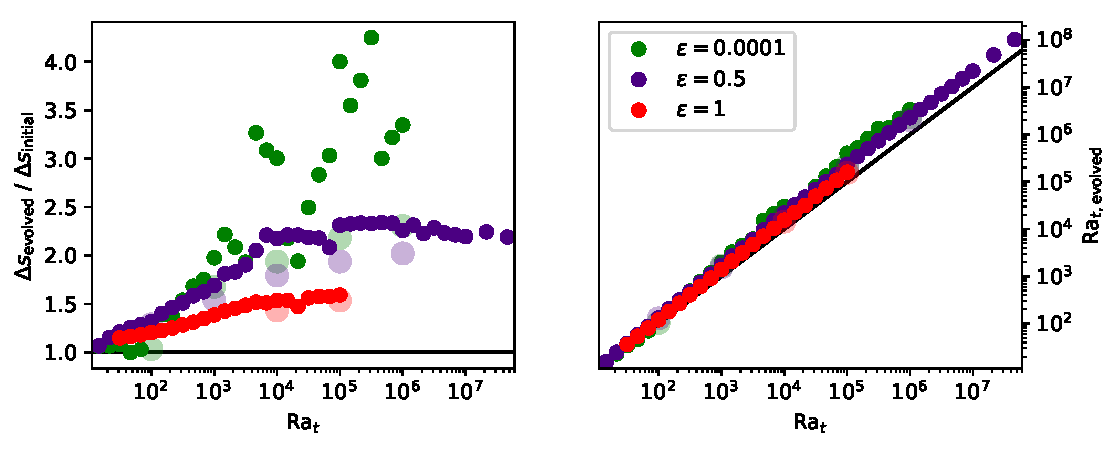
\includegraphics[width=\textwidth]{./figs/delta_S_vs_ra.png}
\caption{ 
	\label{fig:delta_S_vs_ra} }
\end{figure}

\end{document}
